\documentclass[12pt, english]{article}

\usepackage{sbc-template}

\usepackage{graphicx,url,amsmath}

%\usepackage[brazil]{babel}   
\usepackage[latin1]{inputenc}  

     
\sloppy

\title{Social Capital Inequalities among Postgraduate Students and Social Selection Processes}

\author{Neylson J. B. F. Crepalde\inst{1}}


\address{Departmento de Sociologia -- Minas Gerais Federal University (UFMG)\\
  Belo Horizonte, MG -- Brazil
  \email{neylsoncrepalde@gmail.com}
}

\begin{document} 

\maketitle

\begin{abstract}
  This paper aims to discuss social capital inequalities between postgraduate students enrolled in a social sciences program in a Brazilian university. I argue that ``social capital'' concept has been widely and carelessly mobilized which may lead to confusion and spurious conclusions. A solution would be to operationalize social capital with social network analysis. I analyze data from 47 postgraduate students using linear models, stochastic blockmodelling and the Social Selection Model (SSM). The analysis shows that social formations occur mainly from participation in research groups and from methodological perceived habilities. The variable that has the biggest effect on academic productivity is also participating in a research group.
  \\
  \textbf{Keywords}: Social Capital; Social Network Analysis; Social Selection Model.
\end{abstract}
     
%\begin{resumo} 
%  Este meta-artigo descreve o estilo a ser usado na confecção de artigos e
%  resumos de artigos para publicação nos anais das conferências organizadas
%  pela SBC. É solicitada a escrita de resumo e abstract apenas para os artigos
%  escritos em português. Artigos em inglês deverão apresentar apenas abstract.
%  Nos dois casos, o autor deve tomar cuidado para que o resumo (e o abstract)
%  não ultrapassem 10 linhas cada, sendo que ambos devem estar na primeira
%  página do artigo.
%\end{resumo}


\section{Introduction}

The idea of a fully egalitarian world is an impossible abstraction. As \cite{lin1999building} shows, people are born in an already stratified social space where individuals in different positions have different access, and therefore, different mobilizing capacities of their social capital. This is due to individual positioning in social structures, family socioeconomic background, and other person related attributes. This is no news to sociologists. However, the process of social groups formation is not so acknowledged yet although it is central to understand how the access to social resources is achieved. This has only recently been investigated.

This paper aims to discuss the inequalities that are held within the academic system, specifically within a social sciences postgraduate program in a Brazilian university. To do this, we will focus our investigation in two main aspects: academic productivity and social ties formation. We used data collected online from 47 social sciences psotgraduate students (masters and doctoral). To perform the analysis, we used linear models, social network analysis, stochastic blockmodelling and the highly modern \textit{social selection model} (SSM).

This research has the merit of presenting new data and new evidence on the subject and it also operationalizes the concept of social capital in a different and more straightforward way that we see in the literature, i.e., with formal relational data.

\section{Social Capital and Inequalities}

\cite[p. 35]{lin1999building} defines social capital as ``resources embedded in a social structure which are accessed and/or mobilized in purposive actions''. This standpoint leads to three other fidings: first, that there are resources embedded in a social structure. Second, individuals have different accessibility to these resources and, third, they can mobilize this resources in purposive actions. For the purposes of this paper, this definition is sufficient as it accounts for the inequalities that we aim to investigate.

\cite{portes1998social} presents an excellent review on the origin and applicability of social capital in sociology. So does \cite{higgins2005fundamentos}. The later considers three conceptualizations of the term, namely one by Putnam, another by Fukuyama and another by Portes. Putnam investigates the democratic institutions and, for him, social capital is important because ``it is regarded as the source from which spring cooperative interactions that express themselves in different forms of association of the civic community'' \cite[p. 63]{higgins2005fundamentos}. Social capital in this context is related to some specific characteristics of social organization that make the joint action possible, such as norms, trust and symbolic systems.



\begin{quotation}
	Putnam's analysis on social capital as an explaining factor of civic community, which constitutes the context for good institutional performance, concludes with the idea that the stocks of trust, norms and systems of participation tend to be cumulative and reinforce themselves mutually. Virtuous circles are created that result in social balances with high levels of cooperation, reciprocity, civism and collective well-being, characteristics that define civic community. \cite[p. 67]{higgins2005fundamentos}
\end{quotation}

On the other hand, to Fukuyama, ``social capital is an acting and informal norm that promotes cooperation among two or more individuals'' \cite[p. 67]{higgins2005fundamentos}. This can be simply a reciprocity or a huge complex system like Christianity. Every other aspect related to social capital such as norms, trust, etc. are resulting epiphenomena, not constitutive parts of it. According to this author, social capital assumes an economic and a political function reducing transaction costs on formal negotiations and acting as a counterweight to excessive individualism. In Fukuyama's point of view, it emerges from repeated games of the prisoner's dilemma.

\cite{portes2000two} anchors his discussion of social capital on two authors, namely, Bourdieu and Coleman. To Bourdieu, in very general lines, people build their relations taking into account the benefits they could obtain later. Coleman, on the other hand, focus on social capital as social control source.  The author's main focus to show how this concept has been poorly managed giving space to a great amount of confusion and spurious conclusions. To do this, after reviewing in detail both Bourdieu's and Coleman's perspectives on the subject, he analyzes the educational attainment of immigrant children. Social capital indexes are operationalized in these terms:

\begin{quotation}
	Closure of parental networks is measured by the number of parents of child's friends known to her or his parents; parental school involvement is a composite index of parent's participation in school activities and frequency of meetings with school staff about their child's academic progress. The content of these items correspond closely to Coleman's conceptual description of social capital. \cite[p. 7]{portes2000two}
\end{quotation}

Up to this point, it is easy to perceive that the concept is operationalized in a variety of ways in the literature. In fact, \cite[p. 2]{portes2000two} states that ``much of the controversy surrounding social capital has to do with its application to different types of problems and its use in theories involving different units of analysis''. However, since the 1970's, social capital has been conceived within a theoretical framework that accounts both for the structured and the stochastic parts of social life. In this sense, recent researches developed under the relational paradigm in the social sciences pinpoint to the relevance of the mobilization of tangible and intangible resources from imediate social structure of each individual to the possibility of social mobility. In his most famous article ``The Strength of Weak Ties'', \cite{granovetter1973strength} showed the importance of ``distant'' contacts to have access to new information. According to him, ``from  the  individual's  point  of  view,  then,  weak  ties  are  an  importante resource in making possible mobility opportunity'' \cite[p. 1373]{granovetter1973strength}.  In another work, \cite{granovetter1995getting} operationalized the social capital concept magisterally to explain the success within the labor market. He shows that most of the first jobs were obtained through a weak tie. For \cite[p. 470]{lin1999building}, ``the strength of weak ties might lie in their accessing social positions vertically higher in the social hierarchy, which had the advantage in facilitating the instrumental action''.

\cite{erickson2001good} develops her paper in close dialogue with Granovetter. She investigates the effect of social capital on the hiring process focusing both on employee and employer. Social capital here is regarded as the diversity and extension of personal network of the individuals. The author states that social capital can be desirable, irrelevant or undesirable. ``From an employer's point of view, employee social capital can be an asset if used for the  firm but a threat if used by the employee to set up another rival firm, or used by the employee after defecting to another firm'' \cite[p. 131-2]{erickson2001good}. According to the author, ``looking  at  the  social  and  human  capital  that  workers have,  and  the  level  and income  of  the  jobs  they  have,  will show whether good networks make their own contribution to getting a better job'' \cite[p. 133]{erickson2001good}. The main point of the article is that regardless of the contact point by which the job was taken, having a good social capital will lead to better jobs and better pay.


\section{Data and Methods}

In conducting this research, data from 47 postgraduate students was collected through an online survey in May, 2016. This sample corresponds to 60\% of the total number of students enrolled in a postgraduation program at a Brazilian university and it is representative of the total. Therefore, for the purpose of the analysis conducted here, we will assume this group as a ``complete network''.

The developed questionnaire had four parts.The first was an invitation and an agreement term with which the subjects must have agreed to proceed to the questions. In the second part, the subjects were questioned about personal and socialeconomic information. In the third part, they were questioned about their academic life, productivity and impressions. In the last part, the sociometric part, they were present to the complete list of grad colleagues and they were asked to indicate persons regarding 6 issues: scientific collaboration, paper reviewing, theoretical and methodological advisement, friendship and professional indication\footnote{The questions used were: (1) With which of these colleagues did you write or publish a scientific work?; (2) To which of these colleagues did you ask to revise a paper?; (3) If you had a theoretical doubt, whom would you ask for help?; (4) If you had a methodological doubt, whom would you ask for help?; (5) Which of these colleagues do you get together on social occasions?; (6) If you knew about a job vacancy in your acting field, which of these colleagues would you indicate?}. The sociometric questions generated the 6 networks in Figure \ref{six-networks}.

\begin{figure}[!ht]
	\centering
	\label{six-networks}
	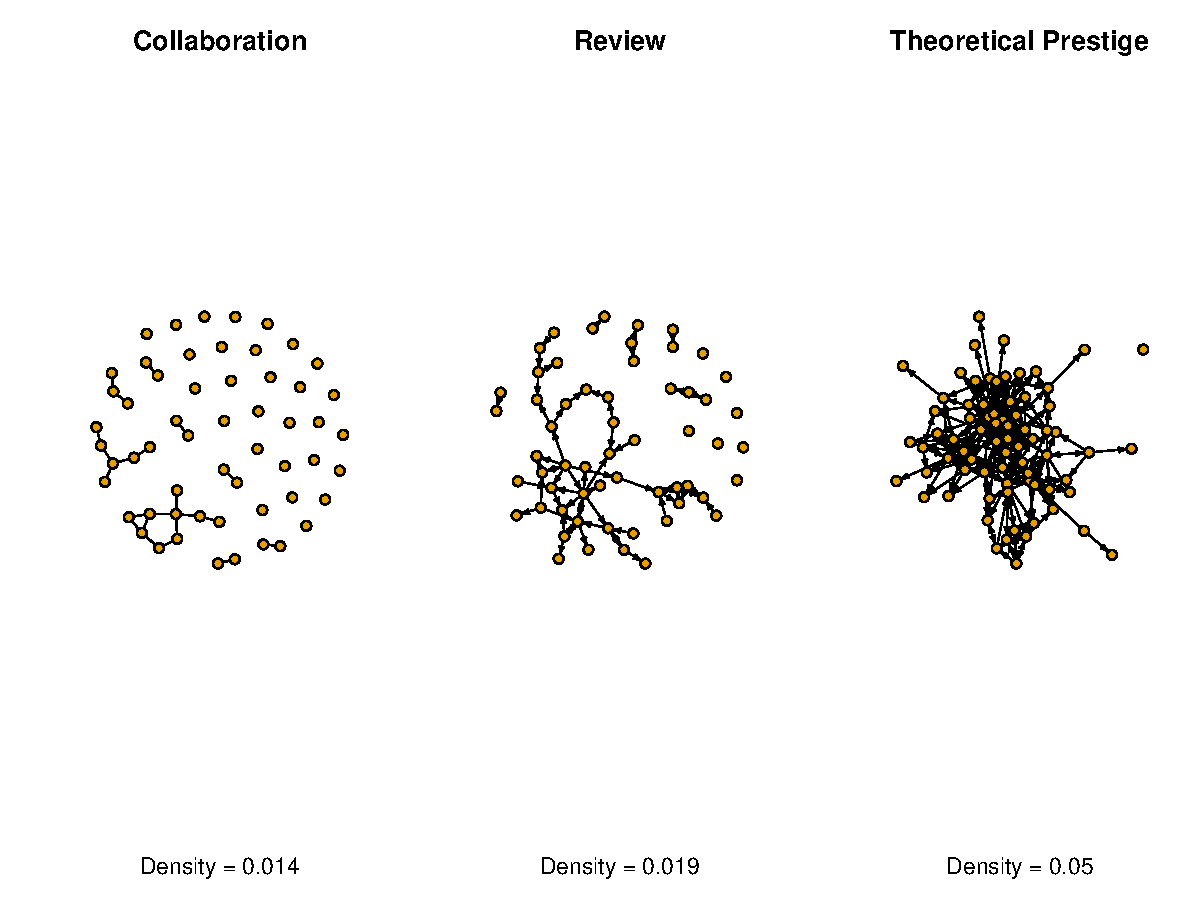
\includegraphics[scale=0.75]{redes1.pdf}
	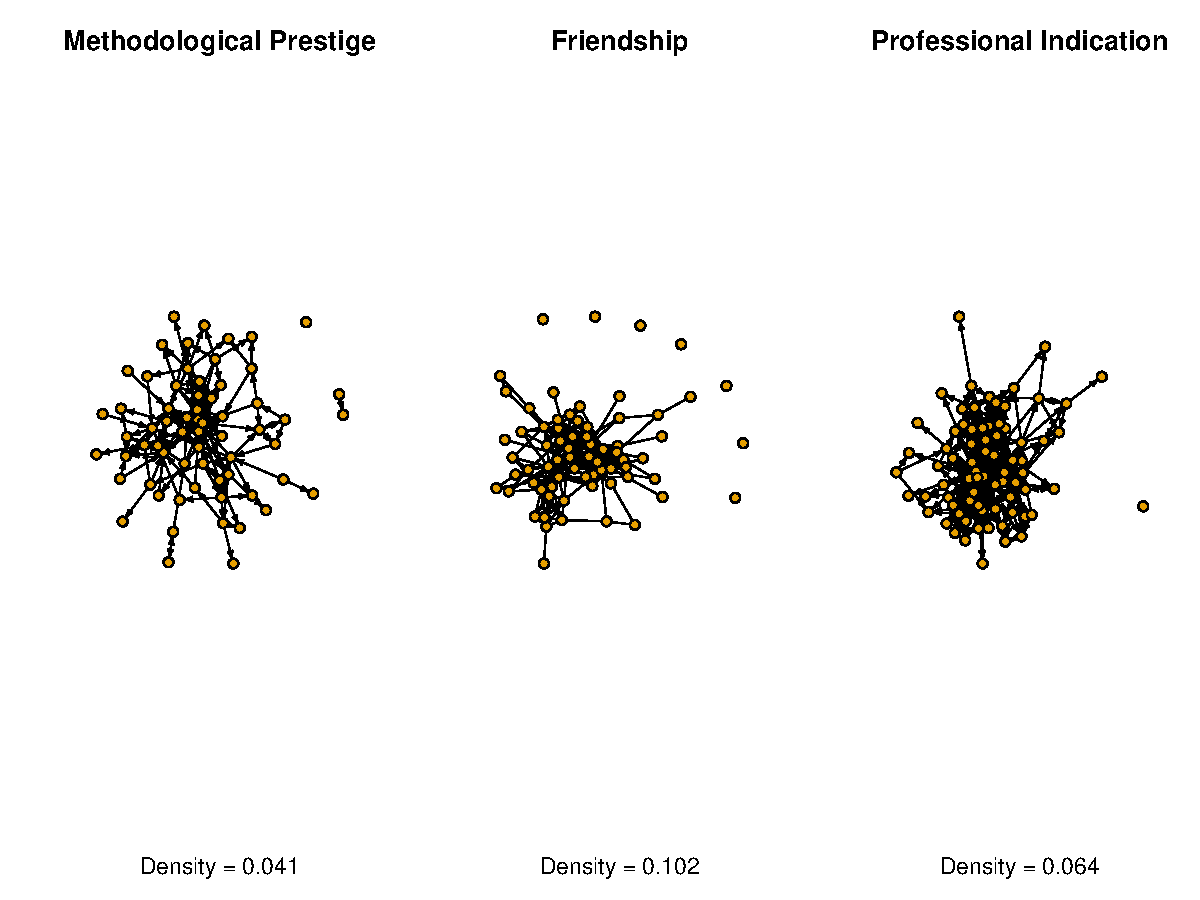
\includegraphics[scale=0.75]{redes2.pdf}
	\caption{Six Networks}
\end{figure}

To perform the analysis, social network analysis metrics were used as well as a statistic model from the \textit{exponential random graph models} family, or p* models \cite{robins2007introduction,lusher2013exponential,lazega2014redes}. This models were developed specially to deal with the observations independence problem. Classic statistical models assume that observations are independent one from another. This is not the case when one is working with network data. ``The fact that I choose Peter as a friend is not necessarily independent of the fact that I also choose Paul because they can be friends with each other'' \cite[p. 76]{lazega2014redes}. \cite{lazega2014redes} state that a tie presupposes a triad which leads to dependency among observations.

The p* model can be defined by

\begin{equation}
Pr(Y=y) \quad = \quad \left(\frac{1}{k}\right) exp \left\{ \sum_{A} \eta_A g_A (\textbf{y}) \right\}
\end{equation}

where Y is the theoretical estimated graph, y is the observed graph, $\sum_{A}$ is the summation of all configurations \textit{A},  $\eta_A$ is the estimated parameter corresponding to the configuration \textit{A}, $g_A(\textbf{y})$ is the network statistic corresponding to the configuration \textit{A} of the graph \textbf{y} and \textit{k} is a constant which ensures the proper probability distribution \cite{robins2007introduction}.

Here, I use an extension of the p* models known as \textit{Social Selection Model} (SSM). The SSM was proposed by \cite{robins2001network} with the goal of accounting for heterogeneity within the social structures using nodal attributes as exogenous covariates. So, in addition to modelling endogenous variables, i.e., network configurations that explain self-organizing processes, the SSM accounts for exogenous variables that also have an effect of structure emergence \cite{wang2016social}. Beyond that, I also analyze the effect of dyadic covariates, i.e., the effect of the existence of an \textit{i--j} tie in another relation network on the existence of an \textit{i--j} tie in the modelled network \cite{robins2013social}.

In the next section, I will analyze how the attributes (exogenous variables) relate to each other, I will describe and present the network measures that are important for this study and I also present the SSM results.

\section{Results}
\subsection{Individual related variables}

If we observe some descriptive statistics of the data in Tables \ref{quanti} and \ref{quali}, we can notice that the respondent students of this postgraduate program have a mean age of 30,32 years and a mean income of R\$2.636,00 (Brazilian reais). Most of them are women, they are predominantly white, 63,8\% do not have a job, 51\% are doctoral students and 70,2\% receive academic scholarship.

% latex table generated in R 3.3.0 by xtable 1.8-2 package
% Fri Jun 10 18:41:28 2016
\begin{table}[ht]
	\centering
		\caption{Descriptive Statistics - Quantitative}
		\label{quanti}
	
	\begin{tabular}{p{4cm}p{4cm}}
			\hline
			Age & Income (R\$) \\ 
			\hline
			Min.   : 23   & Min.   :   0   \\ 
			1st Qu.: 27   & 1st Qu.: 1500   \\ 
			Median : 29   & Median : 2200   \\ 
			Mean   : 30.32 & Mean   : 2636   \\ 
			3rd Qu.: 33   & 3rd Qu.: 3000   \\ 
			Max.   : 43   & Max.   : 8200   \\ 
			\hline
		\end{tabular}
	
\end{table}


% latex table generated in R 3.3.0 by xtable 1.8-2 package
% Fri Jun 10 18:43:47 2016
\begin{table}[ht]
		\small
		\centering
		\caption{Descriptive Statistics - Qualitative (\%)}
		\label{quali}
	
	\begin{tabular}{rrrrr}
			\hline
			Gender & Race & Formal Work & Academic situation & Scholarship \\ 
			\hline
			Female: 63,83   & White: 55.32   & No: 63.83  & Doctor: 06.38   & No: 29.79 \\ 
			Male: 36,17      & Mestizo: 02.13   & Yes: 36.17 & Doctorate Std.: 51.06  & Yes: 70.21 \\ 
			& Dark Skinned: 02.13   &  & Master Std.: 40.43 &  \\ 
			& Black: 04.26   &  & Master: 02.13 &  \\ 
			& Brown: 36.17   &  &  &  \\ 
			\hline
		\end{tabular}
	
	
\end{table}



The subjects were also asked to answer about their perception on their on grades and productivity regarding paper publication. Most students have a good self-evaluation about their grades but a bad one about publishing\footnote{For ``grades'', the perception was measured in a scale from 1 (I have horrible grades) through 5 (I have excellent grades). For ``productivity'', the perception was also measured in a scale from 1 (I do not publish anything ever) through 5 (I am a publishing machine).}. Productivity was measured by the number of published papers, the number of papers presented in congresses and the number of classes given (all since 2014). As a preliminar analysis of the relations between students perceptions (\textit{Grades} and \textit{Pubs}) and their actual productivity (\textit{Papers, Congress} and \textit{Classes}), I correlated this variables. Age and Income were also added to the correlation matrix (Table \ref{correlations}) along with a \textit{productivity score} (\textit{Prod.}) made by summing the productivity variables with weight 2 assigned to published papers.

%\begin{figure}[hbt]
%	\centering

%	\label{self-evaluation}
%	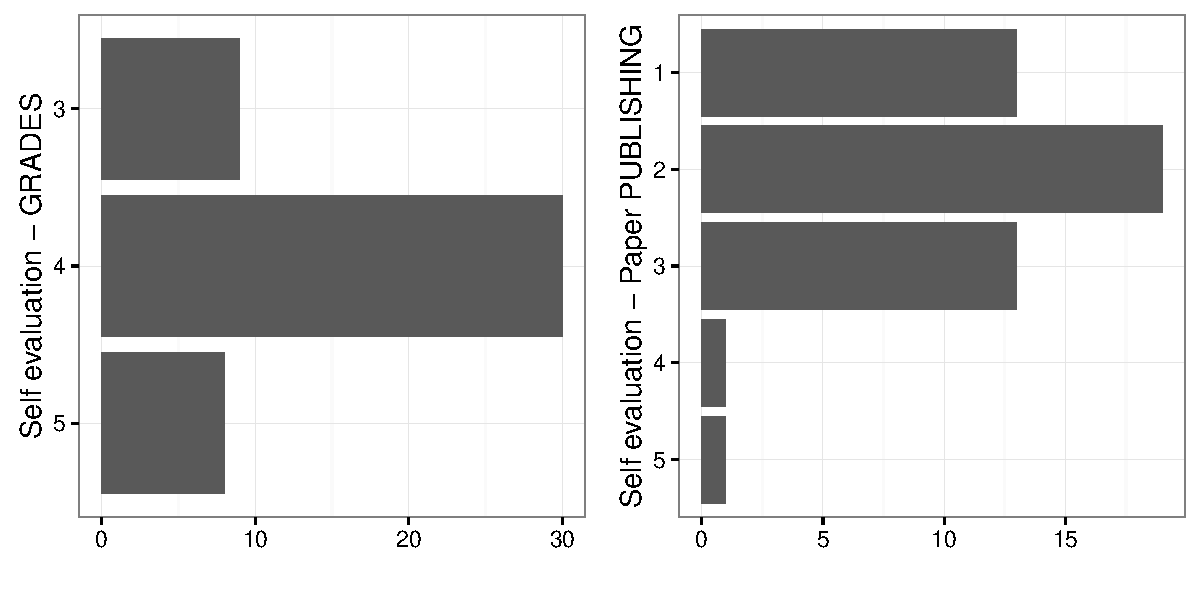
\includegraphics[scale=0.6]{autoavaliacoes.pdf}
%	%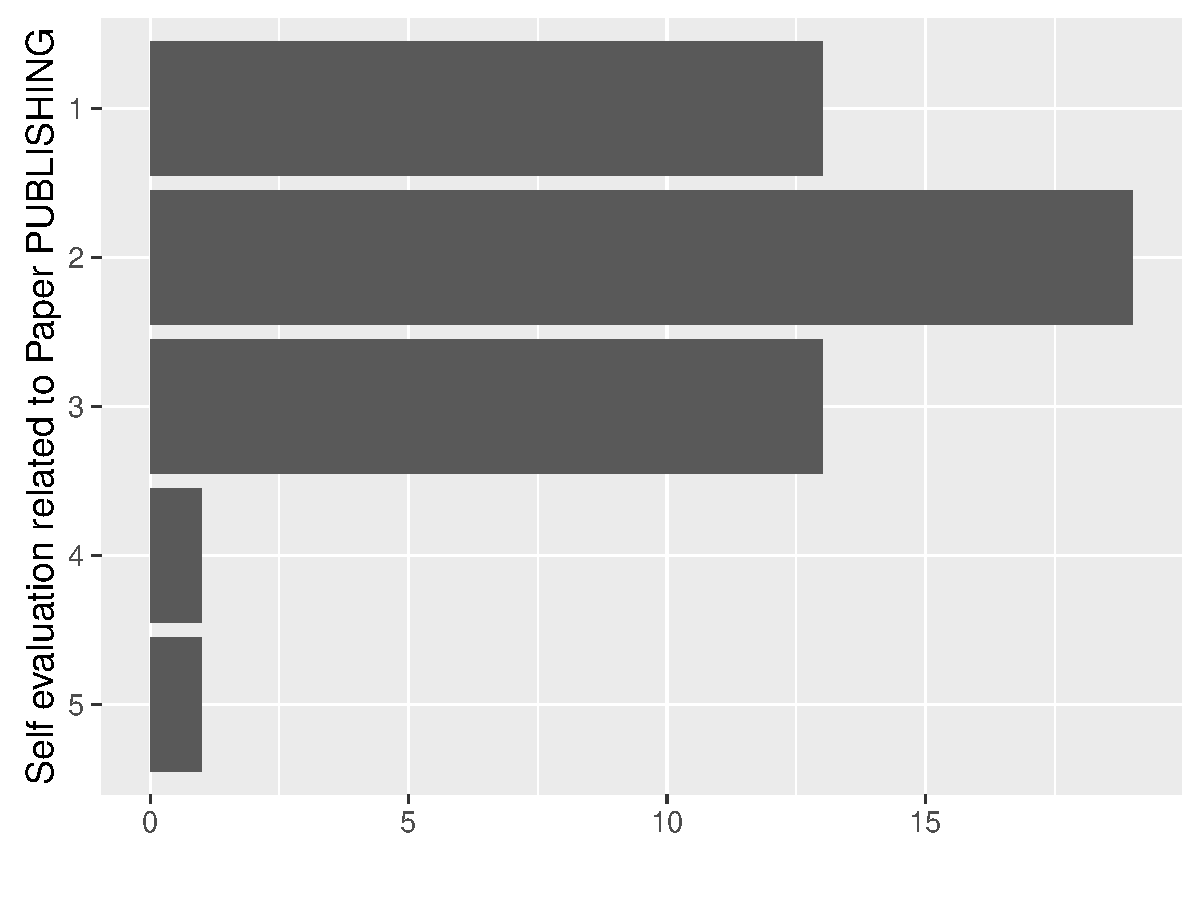
\includegraphics[scale=0.39]{autoavaliacao_publicacoes.pdf}
%	\caption{Self-evaluation}
%\end{figure}


%\begin{figure}[ht]
%	\centering
	
%	\label{productivity}
%	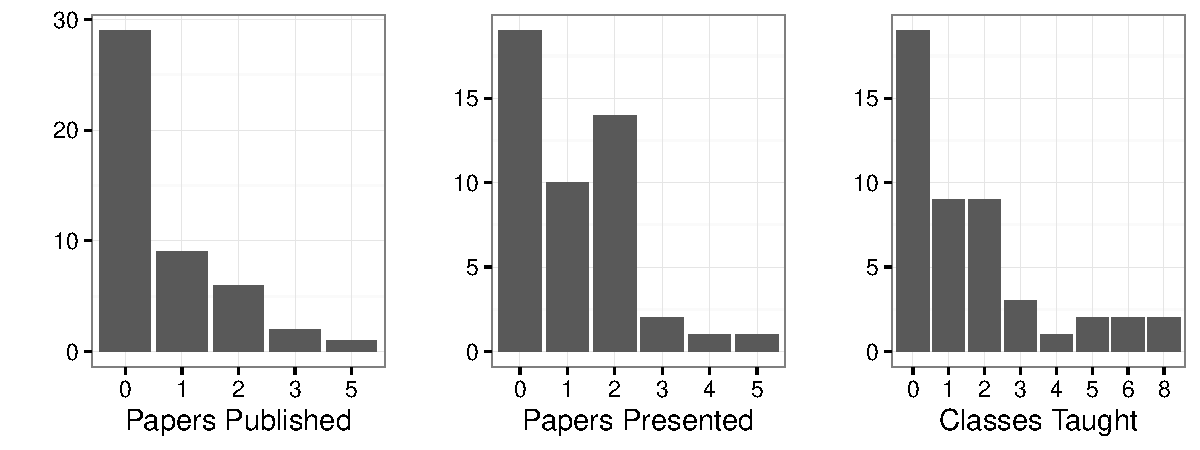
\includegraphics[scale=0.7]{pub_con_classes.pdf}
%	%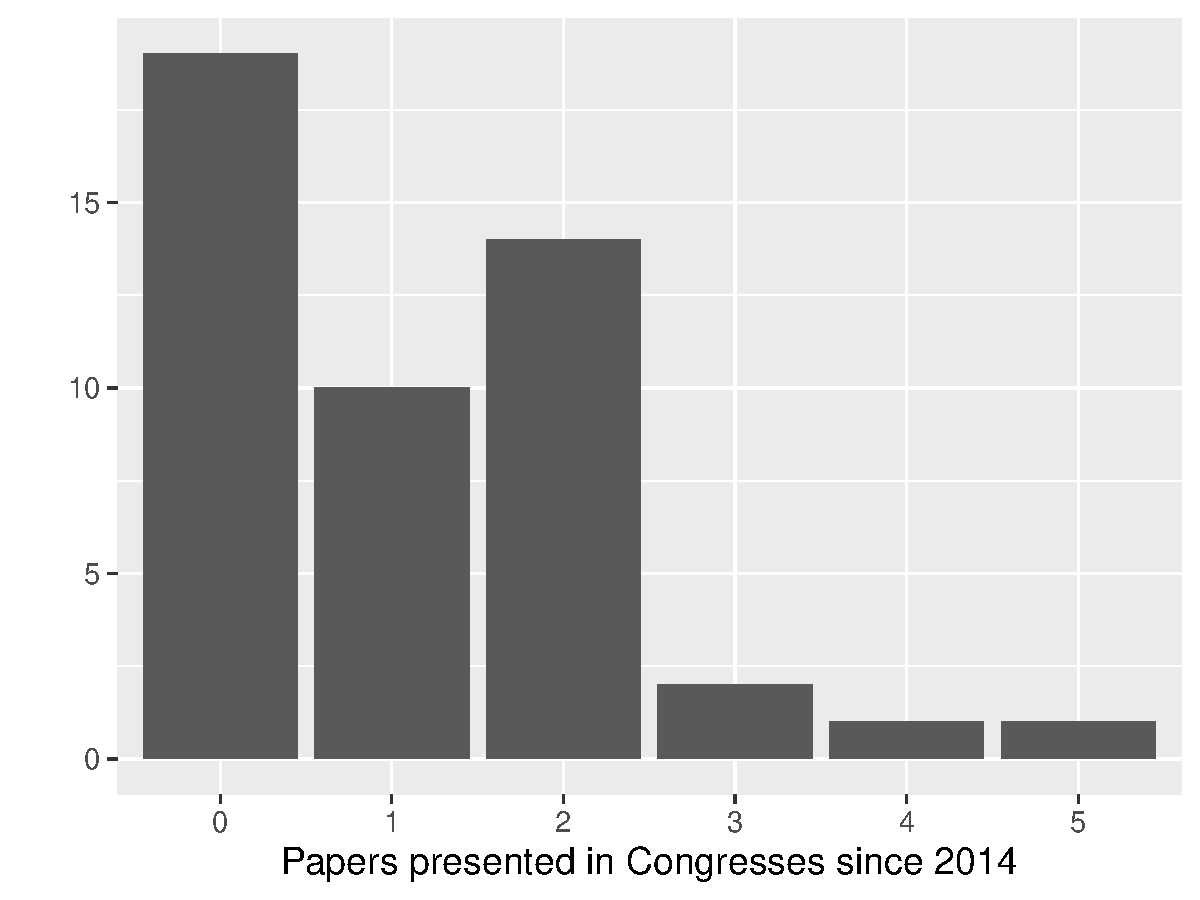
\includegraphics[scale=0.39]{congressos.pdf}
%	%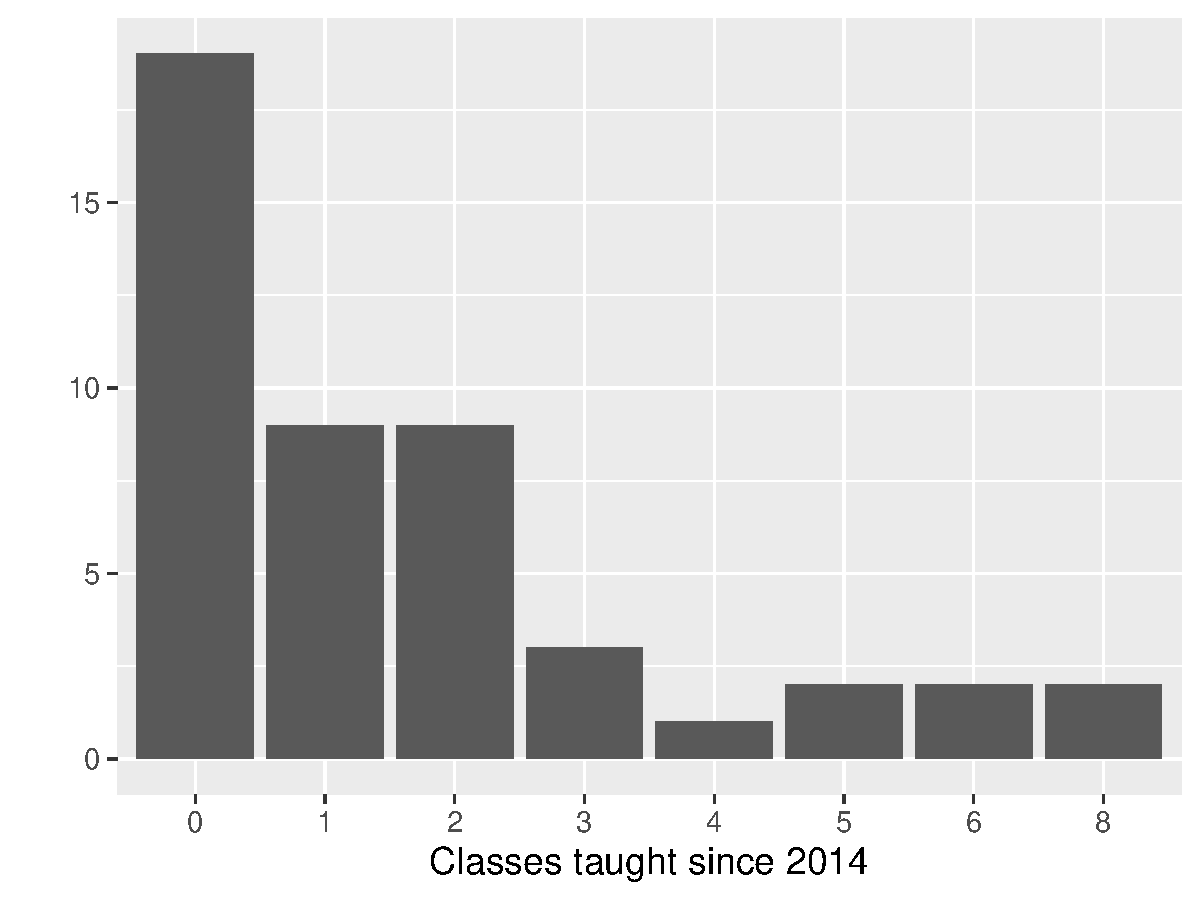
\includegraphics[scale=0.39]{aulas.pdf}
%	\caption{Productivity}
%\end{figure}

% latex table generated in R 3.3.0 by xtable 1.8-2 package
% Fri Jun 10 20:35:58 2016
\begin{table}[ht]

		\centering
		\caption{Correlations}
		\label{correlations}
	
	\begin{tabular}{r|cccccccc}
			\hline
			& Age & Income & Grades & Pubs & Papers & Congress & Classes & Prod. \\ 
			\hline
			Age & 1.00 &  &  &  &  &  &  &  \\ 
			Income & 0.39 & 1.00 &  &  &  &  &  &  \\ 
			Grades & -0.19 & -0.03 & 1.00 &  &  &  &  &  \\ 
			Pubs & 0.09 & 0.16 & 0.32 & 1.00 &  &  &  &  \\ 
			Papers & -0.01 & 0.12 & 0.09 & 0.54 & 1.00 &  &  &  \\ 
			Congress & 0.16 & 0.19 & 0.24 & 0.49 & 0.57 & 1.00 &  &  \\ 
			Classes & 0.21 & 0.45 & -0.16 & 0.15 & 0.18 & 0.07 & 1.00 &  \\ 
			Prod. & 0.16 & 0.37 & 0.04 & 0.53 & 0.82 & 0.65 & 0.66 & 1.00 \\ 
			\hline
		\end{tabular}
	
	
\end{table}

In Table \ref{correlations} we can notice that the variable pairs that have the highest correlation are \textit{Self Evaluation Publications -- Papers}, and \textit{Self Evaluation Publications -- Productivity Score}. Age and Income had very low correlation coefficients with the other variables.

To investigate if age, income, scholarship and occupation have an effect on academic productivity within the studied universe, I estimated two linear models, one by OLS and a Generalized Linear Model with gamma distribution and identity link, with the following specification:

\begin{multline}
\label{linear}
\widehat{Productivity} = \beta_0 + \beta_1ResearchGroup + \beta_2Gender + \beta_3White + \beta_4Self Eval(Pub) + \\ \beta_5Age(centralized) + \beta_6Work + \beta_7Income + \beta_8Scholarship + \epsilon
\end{multline}

The results are presented in Table \ref{linear-coefficients} and a Likelihood test is presented in Table \ref{lrtest}. The Likelihood test shows that model 2 has a better adjust to the data. We are not trying to build a prediction model or making unscrupulous inferences. Therefore, p-values here are irrelevant. We will now analyze the estimated effect of the variables over productivity inside this particular context. Further inferences must respect the self-organizing charasteristics of any empirical social structure. 

What first comes to attention is the big effect that participating in a research group has over productivity.  This is the second biggest effect found on the model and, therefore, a central variable to understand academic productivity. At first, men seem to be more productive than women. A \textit{t test} showed this relation. However, in the GLM, when controlling for the other available variables we find that womem are more productive, \textit{ceteris paribus}. This is very interesting although not possible to deal with here. I intend to deepen into the academic production mechanisms in another work. Also white people seem to be more productive than non-white in this network. Self-evaluation regarding publishing has a big positive effect on productivity. This shows us that students tend to be honest about their own academic performance, nothing more. We can be tented to take hasty conclusions about expectations and productivity but it is very difficult to talk about causality in this case since we have no further information on the mechanisms that involve these variables. All we can affirm is that students expectations are highly correlated with their academic performance. To be working on a formal job seems to reduce productivity which is somewhat obvious. Age and Income have very low effects and, curiously, scholarship has a negative effect. This is also very interesting because it is expected that scholarship students have more time to dedicate to their research projects and, therefore, a higher productivity performance which is not the case. I will come back to this point in the last section.

\begin{table}
		\centering
		\caption{Regression Models}
		\label{linear-coefficients}
	
	\begin{tabular}{l c c }
			\hline
			& Model 1 & Model 2 \\
			& (OLS)   & (GLM -- Gamma) \\
			\hline
			Intercept    & $-1.14 \; (2.17)$     & $0.19 \; (1.88)$      \\
			Research Group (Yes) & $0.86 \; (1.06)$      & $1.52 \; (0.91)$      \\
			Gender (Male)  & $0.43 \; (1.17)$      & $-0.38 \; (0.71)$     \\
			White (Yes)    & $0.70 \; (1.06)$      & $0.79 \; (0.73)$      \\
			Self-eval (Pub)    & $1.93 \; (0.60)^{**}$ & $1.80 \; (0.54)^{**}$ \\
			Age (centralized)     & $0.00 \; (0.12)$      & $0.13 \; (0.10)$      \\
			Work (Yes)  & $-1.69 \; (1.37)$     & $-1.43 \; (0.89)$     \\
			Income     & $0.00 \; (0.00)^{*}$  & $0.00 \; (0.00)$      \\
			Scholarship (Yes) & $-0.52 \; (1.34)$     & $-0.55 \; (0.99)$     \\
			\hline
			R$^2$          & 0.41                  &                       \\
			Adj. R$^2$     & 0.29                  &                       \\
			Num. obs.      & 47                    & 47                    \\
			RMSE           & 3.33                  &                       \\
			AIC            &                       & 238.57                \\
			BIC            &                       & 257.07                \\
			Log Likelihood & -118.29               & -109.29               \\
			Deviance       & 422.34                & 19.16                 \\
			\hline
			\multicolumn{3}{l}{\scriptsize{$^{***}p<0.001$, $^{**}p<0.01$, $^*p<0.05$}}
		\end{tabular}
	
	
\end{table}

% latex table generated in R 3.3.0 by xtable 1.8-2 package
% Fri Jun 24 00:10:53 2016
\begin{table}[ht]
	
		\centering
		\caption{Likelihood Ratio Test}
		\label{lrtest}
	
	\begin{tabular}{lrrrrr}
			\hline
			& \#Df & LogLik & Df & Chisq & Pr($>$Chisq) \\ 
			\hline
			OLS & 10 & -118.29 &  &  &  \\ 
			GLM (Gamma) & 10 & -109.29 & 0 & 18.01 & 0.0000 \\   
			\hline
		\end{tabular}
	
\end{table}

\subsection{Relational Data}

Here, we begin to operationalize the social capital concept as resources embbeded in the social structure. The main purposive action of the postgraduate student in Brazilian academic system is to publish. In the mobilization of one's immediate social structure, this can be facilitated by collaborating, asking for a pair review on a ready article or simply by taking advisement from people that have more theoretical or methodological habilities. Also, popularity and a good social positioning, for example, are powerful social resources. Let us begin the analysis.

%In Figure \ref{degree-distributions}, I present the degree distributions for the six networks.

%\begin{figure}[htb]
%	\centering

%	\label{degree-distributions}
%	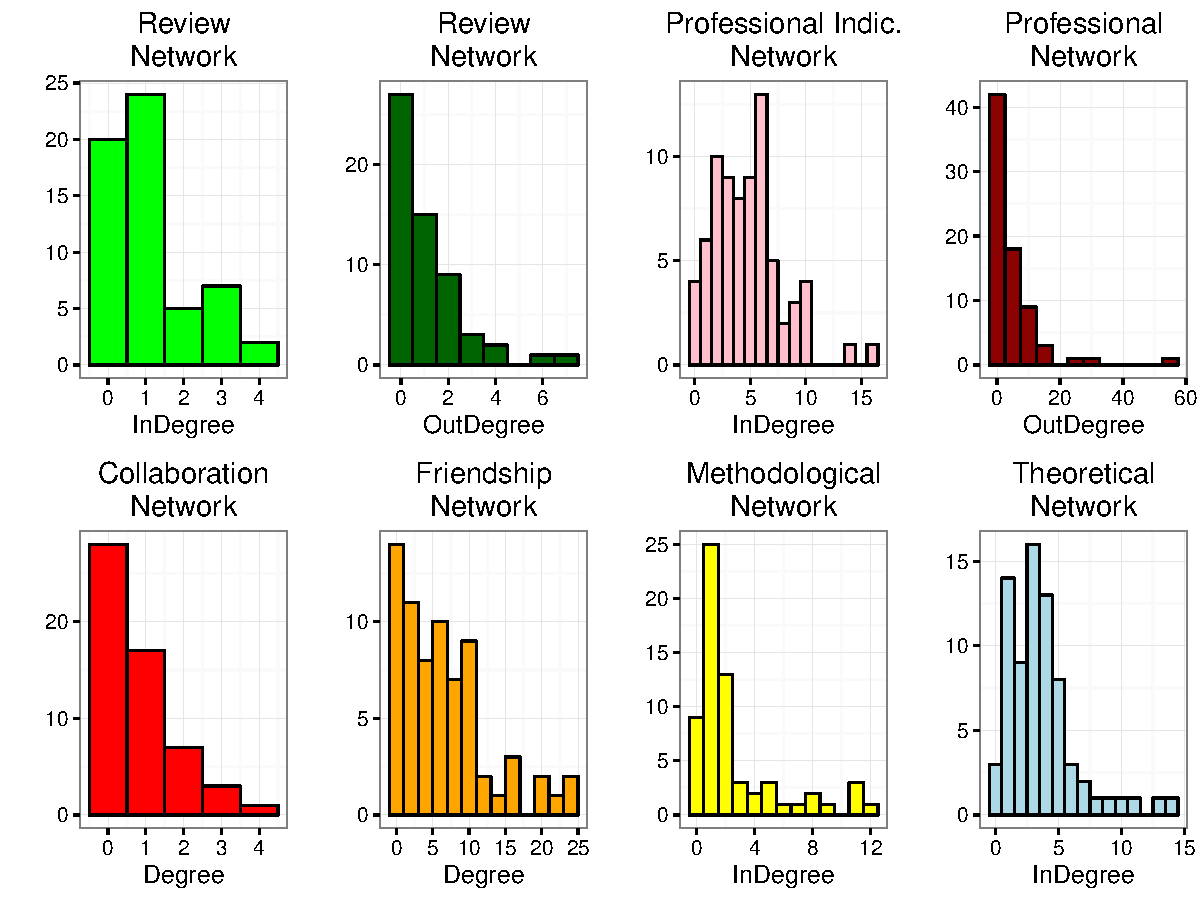
\includegraphics[scale=0.7]{degree_distributions.pdf}
%	\caption{Degree Distributions}
%\end{figure}

The network measures that interest us here are, predominantly, indegree centrality and outdegree centrality which are indicators respectively for popularity and activity. We can notice that Review and Collaboration networks are not so connected; they have a high amout of nodes with degrees 0 and 1. The Professional Indication network is relatively decentralized with popularity and it has some nodes who are extremely active (with more than 20 indications). The Friendship network is also highly decentralized. Regarding the Methodological and the Theoretical advisement, popularity is what is most important for this investigation rather than activity, i.e., who is seen by the pairs as the most competent student regarding methodological and theoretical issues and in what extent this popularity relates with productivity. It is important to observe that the Methodological network is more concentrated than the Theoretical one. The later has more nodes with indegrees 3, 4 and 5 than the former. 

I estimated again the generalized linear model presented in equation \ref{linear} with ``log'' link and the gamma distribution and including centrality measures for the collaboration, review (in) and methodological (in) networks, one at a time; although no one of them had a significant effect, again, the p-value here is not relevant. The exponential coefficients for these measures were $Cent(Collaboration) = 1.17$, $Cent(Review) = 1.10$ and $Cent(Methodological) = 1.00$ showing that people who collaborate tend to be more productive. The same is applied to people who are regarded as methodologically competent.

\subsection{Collaboration and association among postgraduate students}
\subsubsection{Stochastic Blockmodel}

One of the most important concepts of social network analysis is \textit{structural equivalence}. Two individuals are considered structurally equivalent when they present the same relational profile, i.e., the same tie patterns \cite{lazega2014redes,denooy2011exploratory,wasserman1994social}. 

I looked after blocks of structurally equivalent nodes within the Review network. I used the Erdös-Rényi mixture model, a special case of binary stochastic blockmodels. It was fit with the algorithm presented by \cite{daudin2008mixture}. 

%The results for the model are shown in Figure \ref{net-blocks}. 

%and the Review network coloured by block is in Figure \ref{net-blocks}.

%\begin{figure}[ht]
%	\centering

%	\label{blockmodel}
%	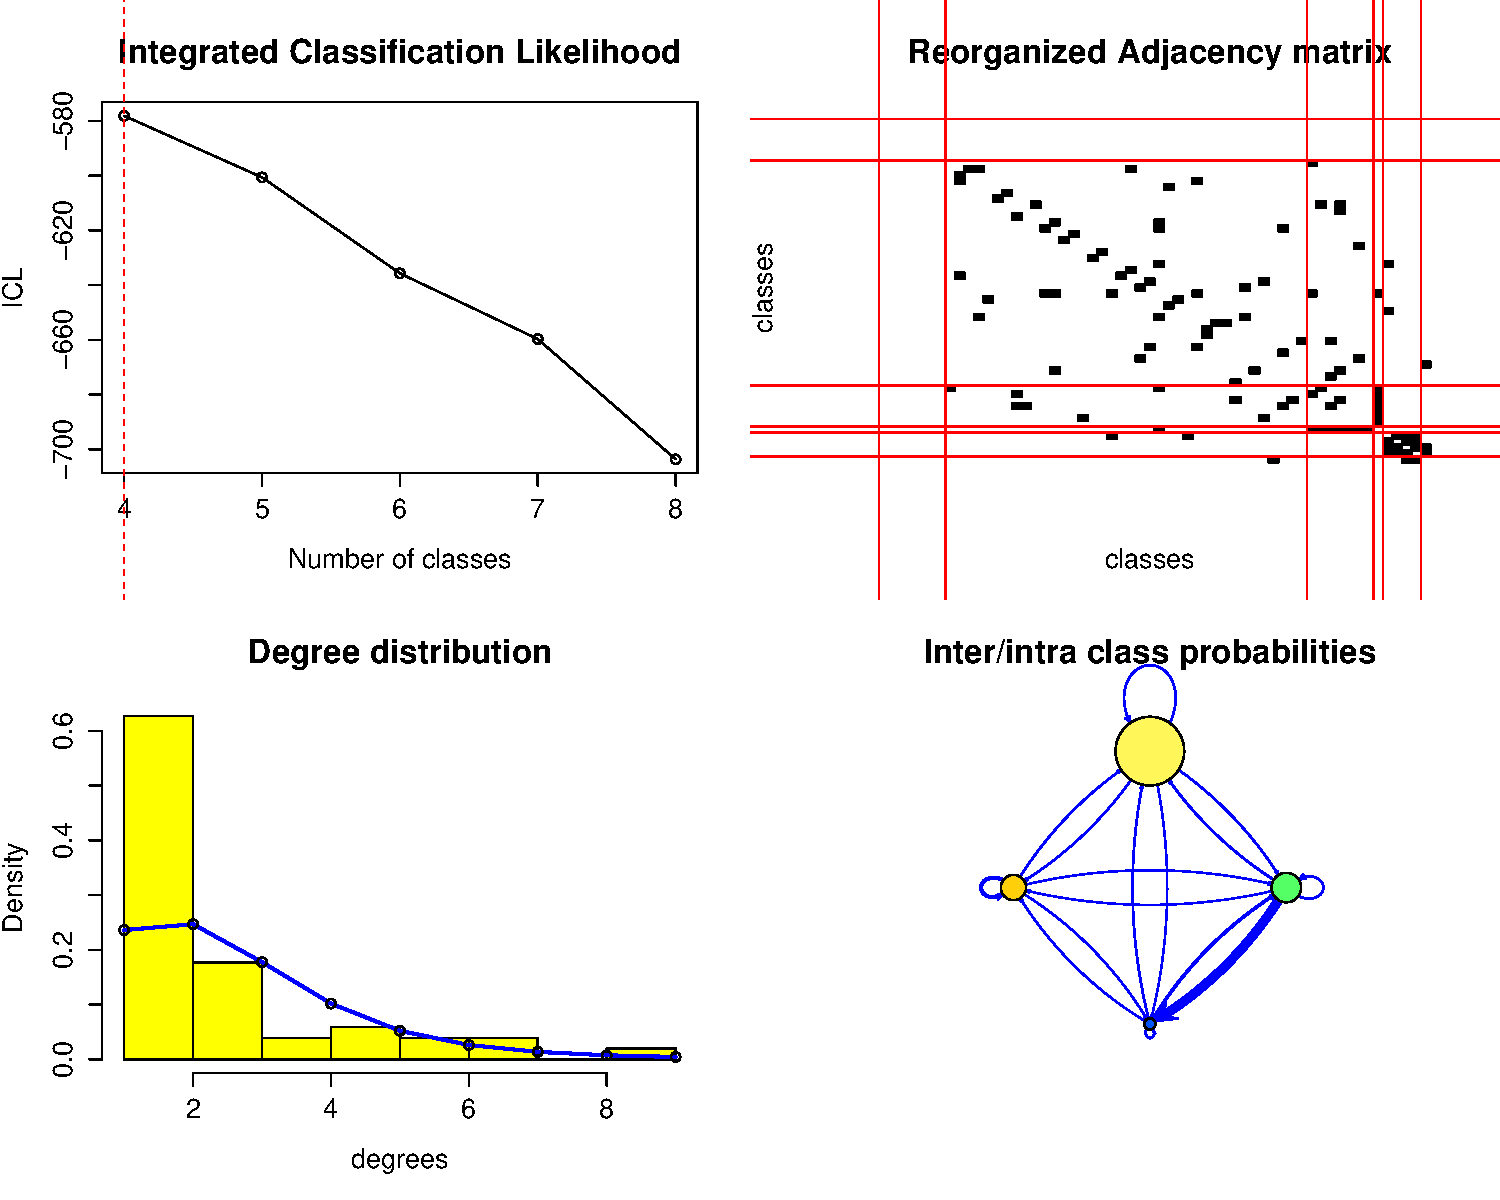
\includegraphics[scale=.5]{block_out.pdf}
%	\caption{Blockmodel results}
%\end{figure}

%\begin{figure}[h]
%	\centering

%	\label{net-blocks}
%	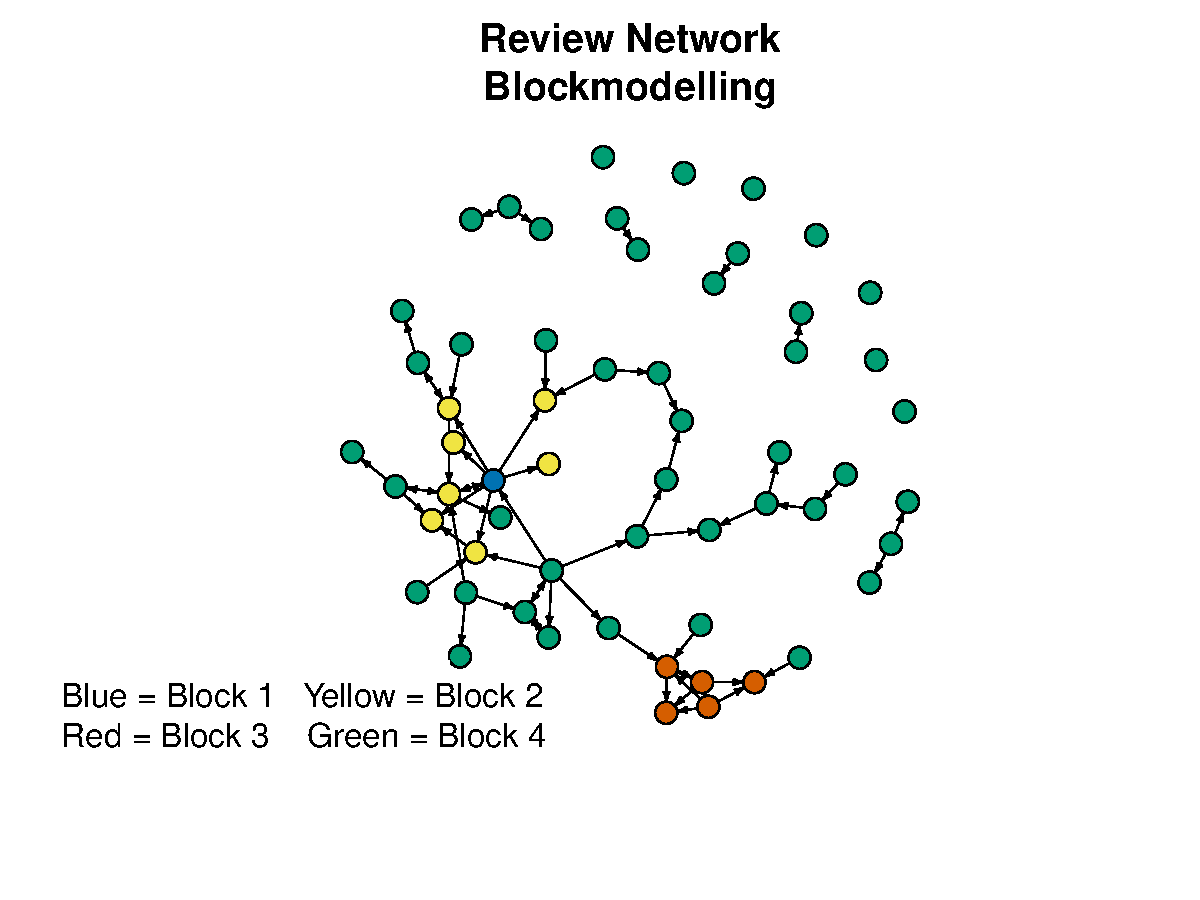
\includegraphics[scale=.6]{net_block.pdf}
%	\caption{Review Network with Structural Equivalence}
%\end{figure}

The algorithm got a best result with 4 blocks. Blocks 1 (two students) and 2 (seven students) are constituted by individuals who are affiliated to two very close research groups. These groups deal with quantitative sociology and social network analysis. Block 3 (five students) shows people who belong to other research group that focus on sociology of crime. The remaining students were allocated to Block 4. The model shows that people within strong research groups tend to be structurally equivalent regarding requests for review.

The blockmodel clustered nodes according to some strong research groups within the program. This shows us that being in a group shapes your relational pattern and, therefore, it is an important feature of social reality. Now, we will focus on the Collaboration network seeking an statistical explanation for its emergence.

\subsubsection{Social Selection Model}

In Table \ref{ergm_colab} are presented the results for the p* models estimated to analyze the Collaboration Network. First I estimated a model only with edges and controlling for the covariate network effects. Then, I inserted three more structure configurations, namely, isolates, triangulation and connectivity to estimate model 2. Model 3 was fit inserting five attribute related statistics, namely, being in the same research group, being of the same sex, being white, the productivity score and income. Statistical significance is measured here by Wald test, i.e., the coefficient will be statistic significant if it is bigger than two times the standard error \cite{lusher2013exponential,lazega2014redes}.

\begin{table}[!h]
	
		\centering
		\caption{ERGM's -- Dependent: \textbf{Collaboration Network}}
		\label{ergm_colab}
	
	\begin{tabular}{l c c c }
			\hline
			& Model 1 & Model 2 & Model 3 \\
			&         & (ERGM) & (SSM) \\
			\hline
			\textbf{Purely structural effects} & & & \\
			Edges  				  & $-4.56 \; (0.28)^{*}$ & $-4.05 \; (1.10)^{*}$ & $-4.22 \; (0.13)^{*}$ \\
			Isolates              &                         & $0.52 \; (0.74)$        & $0.37 \; (0.22)$        \\
			Triangulation (gwesp) &                         & $1.04 \; (0.36)^{*}$   & $1.07 \; (0.29)^{*}$  \\
			Conectivity(twopath)  &                         & $-0.16 \; (0.29)$       & $-0.14 \; (0.15)$       \\
			\textbf{Covariate network effects} & & & \\
			Review net            & $1.81 \; (0.70)^{*}$   & $1.87 \; (0.68)^{*}$   & $2.31 \; (0.14)^{*}$  \\
			Theoretical net       & $0.40 \; (0.66)$        & $0.40 \; (0.65)$        & $0.54 \; (0.14)^{*}$  \\
			Methodological net    & $1.26 \; (0.68)$        & $1.27 \; (0.66)$        & $1.24 \; (0.13)^{*}$  \\
			Professional Indic. net & $0.81 \; (0.52)$        & $0.73 \; (0.50)$        & $0.65 \; (0.23)^{*}$   \\
			Friendship net        & $-0.46 \; (0.67)$       & $-0.50 \; (0.66)$       & $-0.54 \; (0.09)^{*}$ \\
			\textbf{Actor-relation effects} & & & \\
			Same Research Group        &                         &                    & $1.94 \; (0.29)^{*}$  \\
			Homophily (Gender)        &                         &                     & $-0.65 \; (0.12)^{*}$ \\
			Homophily (White)         &                         &                     & $-0.73 \; (0.31)^{*}$   \\
			Absolute Difference (Productivity) &            &                         & $-0.00 \; (0.05)$       \\
			Absolute Difference (Income)       &            &                         & $0.00 \; (0.00)$        \\
			\hline
			AIC                   & 223.33                  & 220.81                  & 220.26                  \\
			BIC                   & 255.15                  & 268.54                  & 294.51                  \\
			Log Likelihood        & -105.66                 & -101.41                 & -96.13                  \\
			\hline
			\multicolumn{4}{l}{\scriptsize{$^*significant$ (Wald test)}}
		\end{tabular}
	
\end{table}

All adjustment measures suggest that model 3 is the one best suited for the network we want to explain. We will focus on it. The edges parameter is often compared to the intercep of a regular regression model. It indicates that this network has a lot less edges than it would be expected in a ``random world''. The isolates and the connectivity coefficients were not significant which indicates us that these are not important configurations for the emergence of this network. Triangulation coefficient indicates that this network has a tendency for group formation. The estimates for the covariate network effects show that all other measured relations have influence on how postgraduate students collaborate. The effect of the Review net is the biggest one which shows us that students who ask for paper review have a lot more probability to actually write or publish in partnership. The second biggest effect is found in Methodological net. This result tell us that students tend to collaborate more with people they see as methodological competent than with they see as theoretically competent. The positive and significative coefficient for Professional Indication net explicits a different and more generic kind of prestige. The Friendship net had a negative and significant estimate showing that these postgraduate students build different relations with regard to friendship and academic work. They tend to write and publish with some people and develop friendship relations with different people, i.e., these two social features do not coincide.

The SSM shows that, again, participating in a research group is a very important variable to understand academic collaboration. The research group big effect tells us that the students have greater probabilities of writing and publishing together within groups. I also tested gender and race homophily; both were refused by model results. Students in this program tend to collaborate with people of different race and gender. I did not find any significant estimates for productivity score and income which shows these are not important variables to explain collaboration ties formation.


\section{Discussion}

James \cite[p. 213]{moody2004structure} stated that the scientific collaboration network in social sciences is moved by research specialty and that ``quantitative work is more likely to be coauthored than non-quantitative work''. In this research we found the same pattern with the difference that it was not the research specialty itself that connects students but, essencialy, the research groups. This is very clear from both the blockmodel and the SSM results. The main cement that glues this postgraduate students together in scientific collaboration is the research groups. Furthermore, the second main aggregator was methodological advisement. The SSM showed that methodological habilities lead to collaboration more than theoretical ones. This is in consonance with \cite{moody2004structure}'s findings about quantitative work. In fact, the research groups that appear in the blockmodel are essentially quantitative researchers.

The linear models did not present big productivity differences by gender, race or income. In this sense, a postgraduate program seems to provide equal opportunities for all its students, once they are in. The models pointed for the centrality of research groups to productivity.

A quite amazing finding is that scholarship students are less productive than non-scholarship ones. This deserves deeper investigation for it contrasts all university funding policies. One hypothesis would be that most non-scholarship students work as professors in other universities and, therefore, are more productive considering the amount of classes to give and final works to orient. That was not the case since most non-scholarship students are not working. Also, that hypothesis is not in agreement with the linear models results which show that, on average, students who work are less productive than those who do not. This subject is out of the scope of this paper and I will limit myself to point the relevance of further investigation.

Finally, I hope to have shown the strength of social network analysis on the operationalization of social capital. Here I could deal with this very same concept, i.e., ``resources embedded in a social structure which are accessed and/or mobilized in purposive actions'' \cite[p. 35]{lin1999building} in a more straightfoward and objective way using social network analysis. We can actually visualize the social structure and mathematically measure popularity, social positioning and social roles. Studies on social capital inequalities would gain a lot with the use of this methodological framework and a more reflexive way of thinking on social capital.

\bibliographystyle{sbc}
\bibliography{BIBSEA}

\end{document}
